%%PART 3 : LA DIFFICULTE
\subsection{Difficulté}
Dans son livre \emph{La cigale : jeux, vie et utopie}, le philosophe Bernard SUITS indiquait : \begin{quote}{“Jouer consiste à tenter volontairement de surmonter des obstacles inutiles”}.  \end{quote}
		
	\subsubsection{Définition et propriétés}
La difficulté s’inscrit comme l’un des principes de base dans la création d’un jeu vidéo, et l’un des mécanismes pourvoyeurs de plaisir principaux de celui-ci. Il n’y en en effet pour un joueur rien de plus frustrant qu’un jeu à la difficulté inexistante ou à l’inverse tout bonnement injouable de par sa difficulté excessive. \paragraph{}

Dans sa thèse, Guillaume Levieux [Levieux, 2011]\cite{Levi11} propose de définir la difficulté d’un jeu vidéo comme l’effort fourni par le joueur pour atteindre ses objectifs. La difficulté d’un jeu n’est pas une donnée stable et suit un processus qui doit être en constante évolution. Le niveau du joueur varie en effet au fil du jeu, du fait de son expérience et de son apprentissage, et la difficulté doit donc s’adapter. 
La difficulté n’est donc en fait pas une propriété du jeu mais la valeur de la relation entre le jeu et le joueur. Or en jouant, le joueur progresse, découvre l’univers du jeu et parfait sa connaissance de la mécanique du jeu, devient capable d’heuristiques pour prévoir les conséquences de ses actions, augmente ses capacités de coordination oculo-manuelle et sa vitesse de réalisation des actions. La difficulté est donc variable, et tend à diminuer au cours du temps. La figure \ref{evolution_difficulte} illustre l'évolution de la difficulté d'un jeu au cours du temps.\\
Notons que le niveau du joueur peut aussi varier à la baisse, si il ne joue pas au jeu pendant un certain temps par exemple.

\paragraph{}L’effort du joueur n’est pas directement mesurable à partir de l’historique de jeu, mais ses résultats le sont. Le problème c’est que l’effort n’est pas normalisé et dépend de chaque style de jeu. La difficulté réside donc dans une relation entre un joueur et le défi qu’il doit relever. La difficulté est en effet relative aux capacités des joueurs : nous n’éprouvons pas tous les mêmes difficultés pour les mêmes jeux ni aux mêmes endroits. Ce qui signifie qu’il faut définir le niveau de capacité des joueurs pour évaluer le niveau de difficulté du jeu.\\
La difficulté d’un problème n'est donc pas uniquement sa complexité : c’est un point de vue humain sur un problème. Une solution est de mesurer les échecs et leur évolution dans un jeu, le taux d’échec étant le résultat visible du niveau de difficulté pour une personne.\\

G. Levieux précise donc dans sa définition de la difficulté, qu’il est important de prendre en compte son aspect relationnel avec le joueur et introduit alors les notions de difficulté absolue et relative (figure \ref{evolution_difficulte})~:
	\begin{itemize}
		\item la difficulté absolue d’un jeu décrit l’effort que doit fournir un joueur type, aux capacités statiques, pour atteindre les objectifs que son gameplay propose. 
		\item la difficulté relative d’un jeu décrit l’effort que doit fournir le joueur, dont les capacités évoluent tout au long du jeu, pour atteindre les objectifs que son gameplay propose.
	\end{itemize}
\paragraph{}Pour maintenir la difficulté relative du jeu, il est donc nécessaire d’augmenter la difficulté absolue du jeu en fonction de l’évolution des capacités du joueur.

\begin{figure}[!htbp]
	\centering
	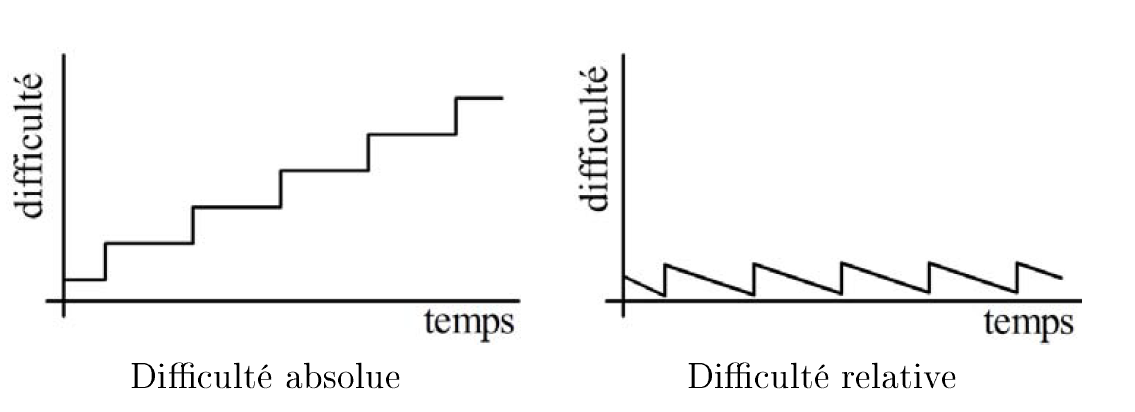
\includegraphics[width=11cm]{images/evolution_difficulte.png}
	\caption{Évolution de la difficulté d'un jeu au cours du temps, Levieux 11\cite{Levi11}}
	\label{evolution_difficulte}
\end{figure}

\paragraph{}La difficulté augmente si l’on resserre les contraintes et délais d’exécutions des actions, si on ajoute de nouveaux éléments qui augmentent la complexité du système ou si l’on découvre une nouvelle partie de l’univers demandant ainsi une appréhension du système plus étend. A l’inverse, la difficulté tend à baisser pour le joueur qui travaille son habileté, ou enregistre le mécanisme de nouveaux éléments ou parties du jeu.

		\subsubsection{Types de difficulté}
Lorsqu'on pense aux jeux vidéo, on envisage naïvement deux types de difficultés : la difficulté de compréhension, et la difficulté d’exécution. Autrement dit, des jeux où il est difficile de savoir ce qu’il faut faire, et d’autres où il est difficile de réussir à le faire. En fait, tout jeu relève à la fois des deux types de difficultés, du moins dans une certaine mesure. C’est d’ailleurs un moyen de différencier un jeu \gls{casual} (un peu des deux difficultés) d’un jeu \gls{hardcore} (une des deux ou les deux, mais bien plus conséquentes). Cependant, ces deux types de difficultés ne s’opposent pas de manière binaire. Les jeux à haute difficulté d’exécution vont souvent être des jeux basés sur un gameplay classique mais en une version très difficile et poussée, alors que les jeux à haute difficulté de compréhension vont relever soit de leur propre genre, soit d’un genre nouveau unique.

\begin{figure}[!hbtp]
	\centering
	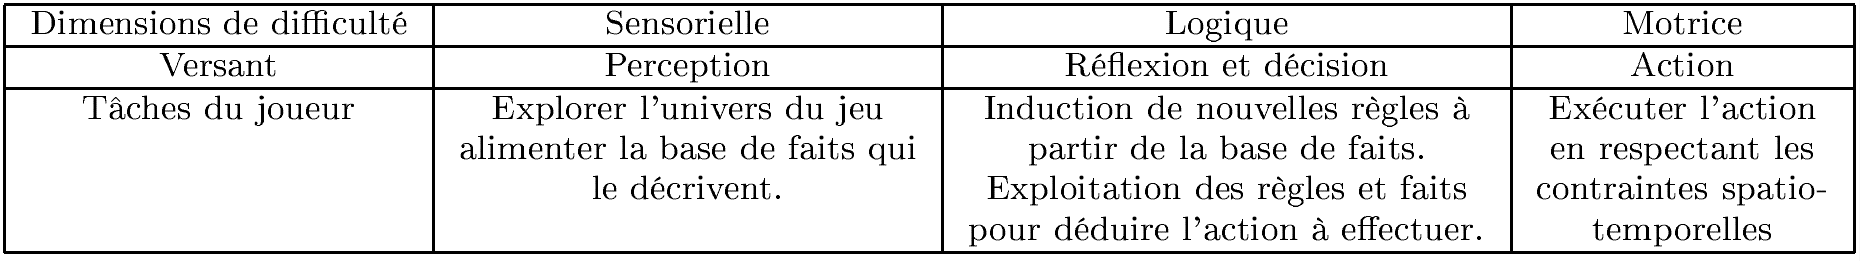
\includegraphics[width=\linewidth]{images/dimensions_difficulte.png}
	\caption{Dimensions de difficulté}
	\label{dimensions_difficulte}
\end{figure}

\paragraph{}
Durant sa thèse, Guillaume Levieux\cite{Levi11} a tenté de mesurer le niveau de difficulté de plusieurs jeux, comme \emph{PacMan}(qui dépend directement de la vitesse de déplacement du joueur et des fantômes). En s’inspirant d’un modèle de traitement de l’information, il a identifié trois niveaux de difficulté~:
	\begin{itemize}
		\item la difficulté sensorielle qui correspond à la perception de l’univers,
		\item la difficulté logique se référant à la compréhension de l’univers,
		\item et la difficulté motrice, en rapport avec l'exécution physique de l’action à effectuer.
\end{itemize}

\paragraph{}Guillaume Levieux \cite{Levi11} définit donc trois types de difficultés dans le jeu vidéo :
	\begin{itemize}
		\item la difficulté sensorielle : décrit l’effort que doit fournir le joueur pour obtenir de nouvelles informations sur l’état de l’univers du jeu. Ces informations nouvelles correspondent à toute information que le joueur ne peut pas déduire des faits et règles logiques qu’il connaît déjà.
		\item la difficulté logique : décrit l’effort que doit fournir le joueur pour exploiter les informations dont il dispose, c’est à dire comprendre le fonctionnement de l’univers par induction, et choisir la prochaine action à réaliser par déduction.
		\item la difficulté motrice : décrit le niveau de précision spatiale et temporelle dont le joueur doit faire preuve lorsqu’il exécute une action.
\end{itemize}
A titre d’exemple, on peut associer un type de jeu par type de difficulté. Les jeux d’aventure se basent essentiellement sur la difficulté sensorielle, les jeux de stratégie sur la difficulté logique, et les jeux d’action sur la difficulté motrice. Bien sur, chaque jeu est composé de chacune des trois dimensions, mais exploitées dans des proportions différentes.
		
		\paragraph{\emph{Punitivité}\\ \quad}
Il s’agit de différencier la difficulté du jeu de la punition en cas d’échec. Ces punitions peuvent être dans l’ordre de sévérité : le respawn instantané (résurrection immédiate), celui avec délai, la sauvegarde libre, le checkpoint (point de contrôle), les vies limitées et la permadeath (mort immédiate et définitive). Ainsi, un jeu peut être très difficile mais peu punitif (\emph{Super Meat Boy}) ou plus facile mais très punitif (\emph{Binding of Isaac}, \emph{Diablo} en mode hardcore). Lorsqu’il est à la fois difficile et punitif, le jeu entre alors dans la catégorie des jeux Hardcore.

		\paragraph{\emph{Le casual et le hardcore}\\ \quad}
Difficulté et punitivité contribuent donc, parmi d’autres facteurs, à créer une relation entre le jeu et le joueur. Plus celles-ci vont être élevées, plus on va s’éloigner du jeu casual pour se rapprocher du jeu hardcore, où un véritable investissement devient nécessaire pour accomplir le jeu. Il nécessite alors un temps d’investissement important ou une concentration soutenue (difficulté), chaque action va peser (punitivité) et demander au joueur de s’investir, à l’inverse du jeu casual.		
		
		\subsubsection{Pourquoi aime-t-on la difficulté?}
			\paragraph{\emph{Chimiquement} \\ \quad}
Le jeu vidéo est capable de fournir aux joueurs des sensations permettant de délivrer au cerveau dopamine ou adrénaline. L’expérimentation du flow state permet aussi au joueur un ressenti qu’il va chercher à renouveler.

			\paragraph{\emph{L’engagement} \\ \quad}
Le jeu vidéo a par ailleurs cette particularité de faire que le joueur va avoir la volonté de recommencer un niveau ou une partie après un échec. Et cette volonté aura tendance à augmenter tant que le joueur n’aura pas atteint son objectif. Cette constatation peut être expliquée par la théorie psychosociale de l’engagement, et plus particulièrement du concept de dépense gâchée. Selon cette théorie, plus on a passé de temps dans une activité, à apprendre quelque chose ou dans une réalisation, moins on est enclin à y renoncer, sous prétexte du temps inutilement passé à s’y consacrer. Dans le jeu “je ne vais pas abandonner après être arrivé aussi loin !”. L’engagement (et l’attachement aux valeurs) est d’autant plus important que l’investissement a été important, que ce soit en terme de temps, d’efforts, de sacrifices, de souffrance, etc.

			\paragraph{\emph{Dissonance cognitive} \\ \quad}
Par ailleurs, l’humain (entre autre) est mal à l’aise et ressent une tension désagréable lorsqu’il est en état de dissonance cognitive. Cette dissonance est ressentie lorsque l’individu est en présence de cognitions (connaissances, croyances ou perceptions de soi ou son environnement) contradictoires ou incompatibles entre elles.
Cet état entraîne un inconfort psychologique, parfois une réaction émotionnelle, qui pousse la personne à penser ou agir. pour rétablir son équilibre cognitif à l’aide de stratégies inconscientes de rationalisation. L’éveil peut prendre bien des formes, la soumission, la rationalisation, la fuite, un comportement ou une action délibérée, la modification de ses croyances, attitudes ou connaissances pour les accorder avec la nouvelle cognition. Dans le jeu vidéo, cela se traduit par une auto justification de la persévérance du joueur, ou un rejet radical de l’activité. On va se trouver des excuses, etc.

			\paragraph{\emph{Découverte et apprentissage}  \\ \quad}
Ces principes sont primordiaux pour un certain nombre de joueurs.  Que ce soit la découverte d’un monde immense, des capacités de son personnage, des mécanismes du jeu ou encore d’un univers particulier, le plaisir réside dans le fait que rien n’est acquis et se découvre à force d’expérimentations et d’échecs. Au fur et à mesure de ses expériences et observations, le joueur va alors suivre une courbe de progression généralement logarithmique très gratifiante qui va l’inciter à poursuivre son apprentissage pour parfaire sa maîtrise du jeu. Cet intérêt est d’ailleurs suffisamment fort pour qu’une certaine communauté de joueurs complète ses connaissances à l’aide de forums, wiki ou vidéos qu’elle aura elle même mis en ligne.

			\paragraph{\emph{Auto-détermination} \\ \quad}
R. Ryan et al propose d’expliquer la motivation du joueur à travers l’auto-détermination. Ils considèrent que les jeux vidéo satisfont des besoins psychologiques et permettent le développement d’un sentiment d’autonomie, de compétence et de connexion. L’autonomie décrit à la fois le fait que l’investissement du joueur est volontaire et que le joueur possède une autonomie au sein du jeu.

			\paragraph{\emph{Auto satisfaction et dépassement de soi} \\ \quad}
Le plus grand plaisir qu’un joueur peut ressentir en jouant à un jeu difficile ou hardcore, est le sentiment d’auto satisfaction lorsqu’il réussit enfin à accomplir son action. A force d’efforts ou d’entraînement, il réussit à réaliser ce qu’il croyait impossible au premier abord, parce qu’il ne comprenait pas comment y arriver ou n’était simplement pas capable de le faire, par manque de techniques, d’imagination ou d’entraînement. Ce dépassement de soi (technique, intellectuel ou physique) est déjà gratifiant en soi, et récompense le long apprentissage auquel s’est adonné le joueur.

C'est la \textcolor{orange}{réussite} d'un challenge \textcolor{orange}{difficile} qui est satisfaisante, et non directement son accomplissement. À l'inverse, une majorité va choisir une difficulté normale plutôt que facile ou difficile, car les gens aiment \textcolor{vert}{faire} quelque chose qui représente un \textcolor{vert}{challenge modéré} : pas le choisir ou le réussir, moins glorieux.

			\paragraph{\emph{L’enjeu} \\ \quad}
C’est aussi un grand pourvoyeur de plaisir. Un fort enjeu va inciter le joueur à ne pas jouer à la légère, à s’impliquer et donc à s’appliquer dans sa partie. On notera que l’enjeu est d’autant plus fort lors de partie multijoueur : les actions d’un joueur peuvent potentiellement influencer l’expérience de jeu de chacun des autres joueurs. En confrontation, il faut arriver à surpasser l’autre joueur, qui va faire de son mieux pour vous en empêcher. En collaboration, où l’erreur de l’un peut alors aussi coûter aux autres. L’enjeu crée alors un sentiment de tension, qui va lui même renforcer l’immersion du joueur.

\paragraph{}Enfin l’intérêt des joueurs pour les jeux difficiles ou réputés comme tels, peut aussi s’expliquer par une certaine \emph{nostalgie}, une forme d’\emph{élitisme} voir de snobisme envers les jeux/joueurs dits casuals, mais surtout aussi par le plaisir ressenti par la réussite d’un défi qui leur est posé. Une forme de frustration idéalement dosée et que l’on a surmontée.

	\subsubsection{Difficulté dans les Serious Games}
Les \glspl{sg} ont la particularité de conjuguer les mécanismes classiques du jeu vidéo à des objectifs sérieux de nature différente. Ces objectifs peuvent être la transmission de connaissances ou de valeurs si la visée est intellectuelle, ou bien un travail sur la forme ou les capacités physiques du joueur. Dès lors, la difficulté du jeu se dote d’une nouvelle composante relative à cet objectif thérapeutique.\\
Dans le cas de \glspl{sg} physiques, qui utilisent des périphériques comme la wii board, la kinect ou le PSmove par exemple, on pourra assimiler cette nouvelle composante à la difficulté motrice déjà définie. A la difficulté de synchronisation oculo-motrice de la main sur le contrôleur, s’ajoutent des difficultés physiques telles que la précision, l’endurance, l’équilibre ou la souplesse.
Dans les jeux dont l’aspect sérieux est intellectuel, l’objectif sérieux peut venir enrichir la difficulté logique du jeu (difficulté de compréhension, de raisonnement, de mémoire).
Dans les jeux sérieux dont le but est une rééducation psychomotrice, il est aussi important d’envisager un nouvel aspect de difficulté de type émotionnel. Il faut en effet prendre en compte l’enjeu médical et la possible fragilité du joueur, dont la progression ou non peut avoir un impact important sur son mental.
\newpage
		
\subsubsection{\emph{Encart proposition \\} Proposition d'une nouvelle composante : la difficulté émotionnelle}
Nous avons vu dans notre recherche documentaire que sont définies trois types de difficultés dans les jeux vidéo. [Levieux, 2011]\cite{Levi11} définit ainsi la difficulté sensorielle, la difficulté logique et la difficulté motrice.

\paragraph{}Il est aussi possible d’envisager une dimension émotionnelle dans la difficulté. Cette difficulté peut se manifester lors de la réalisation d’une action dont la réussite ou non est importante pour le joueur, lors d’une confrontation avec une situation, un problème ou un objet dont le joueur a peur ou le rend particulièrement mal à l’aise par exemple : mise en situation d’une phobie, d’une scène en désaccord avec ses mœurs ou convictions, lui rappelant des évènements difficiles ou traumatisants, etc.
 \paragraph{}
On peut citer l’exemple du jeu \emph{Paper Please}, dans lequel on incarne un employé travaillant à un poste de frontière et qui contrôle l’accès au pays. Dans ce jeu, le joueur sera partagé entre respecter les consignes strictes d’immigration et le caractère émotionnel et personnel des personnes souhaitant entrer dans le territoire avec des histoires et des motivations personnelles, personnes pour lesquelles il lui faudra décider si il autorise ou il restreint l’accès. Cette décision pourra être particulièrement difficile car elle se fera au risque de perdre son emploi et ne plus pouvoir faire survivre sa famille ou d’être en profond désaccord, voir en situation de dégoût, avec soi-même...\paragraph{}
Le joueur peut aussi s’imposer lui-même un certain nombre de contraintes, pour être en accord avec ses principes. Ces contraintes peuvent être d’ordre moral ou éthique (refus de tuer un personnage dans le jeu ou d’effectuer une mauvaise action), ou plus artificiel comme vouloir jouer de manière “Role Play” et donc s’interdire certaines actions ou au contraire s’en imposer d’autres. Ainsi, même si le joueur sait qu’il gagnerait à réaliser une action particulière et qu’il est en mesure d’y parvenir, il ne passera pas nécessairement à l’œuvre. 
\paragraph{}On pourra ainsi citer l’exemple du jeu \emph{Valkyrie Profile}, dans lequel le joueur peut contrôler un personnage principal, ainsi qu’un groupe de personnages secondaires. Durant les phases de combats tactiques, le joueur a la possibilité de sacrifier un personnage secondaire afin d’obtenir une puissance phénoménale, qui se révélera souvent nécessaire d’acquérir tant la difficulté du jeu est élevée. Mais ces sacrifices sont permanents et l’avatar, ainsi que le joueur, devront les assumer et vivre avec la conscience d’avoir tuer ces personnages, ce qui fera évoluer différemment l’histoire.
\paragraph{}
Un autre aspect émotionnel se trouve dans l’acceptation du déroulement du jeu. Dans un jeu multijoueur compétitif ou opposant une IA, si l’adversaire emploie une stratégie ou une technique particulièrement frustrante pour le joueur, celui-ci peut s’en trouver affecté (colère, énervement, mauvaise estime de soi, mauvaise foi). Si cette situation continue ou est répétée, ou bien que malgré une difficulté modérée notre joueur continue de perdre ou de se faire mener en bateau pour une raison ou une autre, la difficulté émotionnelle deviendra telle qu’il pourra préférer abandonner. Cette situation particulièrement fréquente dans les jeux multijoueur en ligne peut mener à ce que l’on appelle couramment un \emph{rage quit}, qui désigne familièrement le fait pour un joueur de quitter une partie en cours sous l'effet de la colère.

\paragraph{}On peut noter que cette difficulté peut en fait impacter directement les trois autres aspects de la difficulté précédemment cités. Un joueur qui aura réellement peur perdra de ses capacités sensorielles, logiques ou motrices par exemple. Cet impact n’est cependant pas systématique : une situation obligeant le joueur à réaliser une action allant à l’encontre de ses principes n’affectera pas ses capacités, mais le joueur hésitera cependant à réaliser l’action qu’il sait nécessaire~; il aura compris la situation, trouvé la solution à sa réalisation et est physiquement capable de la réaliser, mais ne souhaitant pas la faire, différera son exécution, voir l’évitera si possible.

\paragraph{}Dans le cas particulier d’un Serious Game pour la réhabilitation motrice, la difficulté émotionnelle peut se situer dans l’intérêt particulier qu’a le joueur-patient dans l’évolution de sa pathologie. Il est nécessaire en phase de rééducation que le patient soit capable de sentir qu’il progresse afin de garder sa motivation et poursuive son travail. Une confrontation trop fréquente à des gestes qu’il n’est pas encore/toujours pas capable de réaliser parce que trop difficiles, aura pour conséquence de lui rappeler sa déficience et pourra lui faire perdre toute ambition thérapeutique.

\paragraph{}Cette dernière constatation pose la question de savoir si la difficulté d'un jeu vidéo classique est comparable à celle d'un jeu thérapeutique.\\ Le serious game thérapeutique se pose dans un contexte précis, dans lequel les joueurs sont des personnes blessées, physiquement et/ou psychologiquement. Il est ainsi difficile de s'attendre de leur part à des réactions classiques et c'est un facteur dont je pense qu'il est important de tenir compte. Bien doser l'évolution de la difficulté ou des exigences faites envers le joueur est ainsi primordial pour s'assurer du maintien de l'activité, et donc de l'amélioration de son état. Si le joueur se sent biaisé par l'application, à cause d'une difficulté trop importante ou d'une évolution trop rapide, il aura tôt fait de cesser de jouer et le jeu, aussi efficace puisse t-il être par ailleurs, n'aura alors aucun impact.
		
	\subsubsection*{Relation entre les différents paramètres d'un jeu vidéo}
Afin de mieux comprendre pourquoi le jeu vidéo est un média apprécié et comment ses différents paramètres peuvent être utilisés pour des objectifs sérieux, j'ai cherché à trouver le lien entre ces composantes. Dans un contexte de rééducation, on va aussi chercher à connaître quelles théories sont intéressantes pour les thérapeutes, pour qu'ils puissent réaliser un classement par importance pour la thérapie. Le résultat de mes recherches est exposé dans l'annexe~\ref{part_theories}. Comprendre les relations qui existent entre le jeu vidéo et le joueur pourrait aussi permettre de mieux comprendre les mécanismes en jeu et mieux orienter les exercices d'éducation ou de réhabilitation.
\begin{figure}[htbp]
Schéma inspiré des théories comportementales et psychologiques et de concepts mis en place dans les jeux vidéo (voir annexe~\ref{part_theories}).
	\centering
	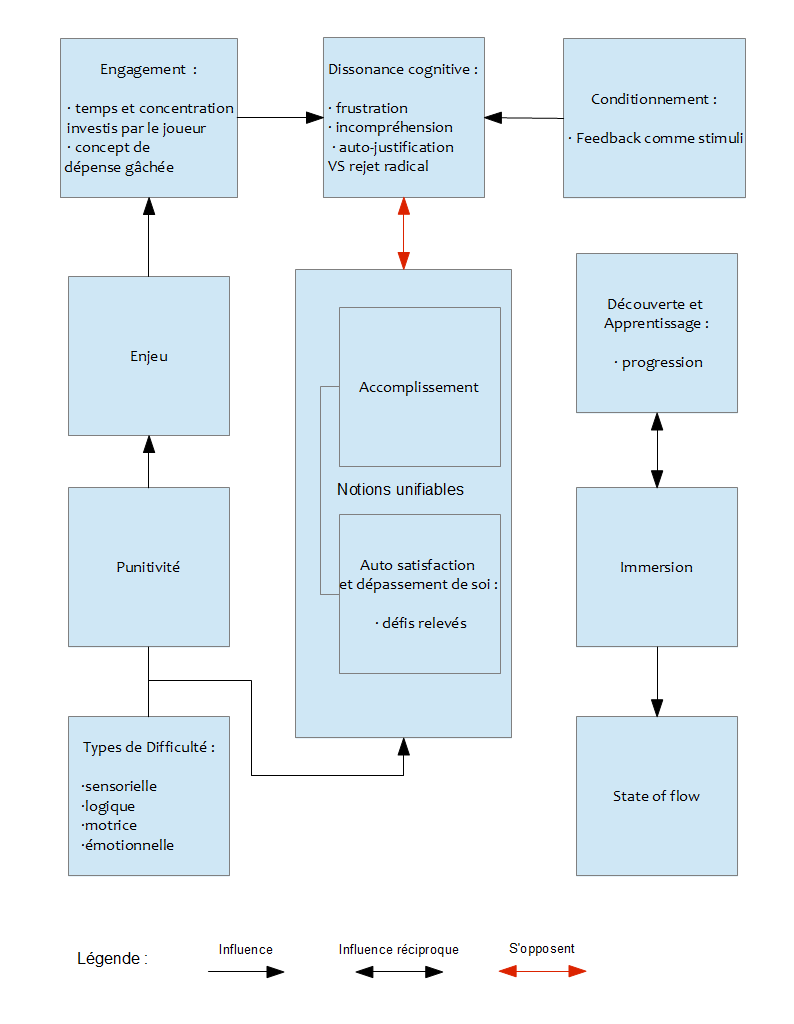
\includegraphics[height=19.6cm]{images/lien_theories}
	\caption{Relation entre les principaux ressorts psychologiques d'un jeu vidéo}
	\label{lien_theories}
\end{figure}			
